\chapter{Basi di dati relazionali distribuite}
\begin{definizione}[\textbf{DDBMS}]
      Un \textbf{DBMS distribuito eterogeneo autonomo} è in generale una
      federazione di DBMS che collaborano per fornire accesso ai dati con livelli
      di trasparenza.
\end{definizione}
Con il termine trasparenza si intende la capacità di un sistema di
nascondere i dettagli di implementazione e di gestione dei dati, fornendo
all'utente una visione unificata e coerente del sistema, spesso nascondendo i gli
aspetti di \textbf{distribuito}, \textbf{eterogeneo} e \textbf{autonomo}.

In base a questi aspetti si definisce una classificazione dei DDBMS per ogni aspetto
e una classificazione per la combinazione dei tre aspetti.

La più importante classificazione che riguarda i $3$ aspetti è:
\begin{itemize}
      \item \textbf{DBMS Distribuiti Omogenei} (DDBMS): C'è distribuzione ma
            nessuna eterogeneità e nessuna autonomia.
      \item \textbf{DBMS Distribuito Eterogeneo}: In questa fase vederemo il
            problema dell'integrazione dei dati.
      \item \textbf{Multi Database MS}: Sistemi totalmente autonomi.
\end{itemize}
\paragraph{Autonomia} L'\textbf{autonomia} di un'architettura dati distribuita
fa riferimento al grado di \textbf{indipendenza} tra i nodi. Possiamo distinguere
diversi livelli di autonomia:
\begin{itemize}
      \item \textbf{di progetto}: ogni nodo ha un proprio modello dei
            dati e di gestione delle transizioni.
      \item \textbf{di condivisione}: ogni nodo sceglie la porzione di
            dati da condividere con gli altri nodi.
      \item \textbf{di esecuzione}: ogni nodo sceglie in che modo eseguire
            le transazioni che gli vengono inviate.
\end{itemize}
Partendo da questa classificazione possiamo definire diversi tipi di DBMS autonomi:
\begin{itemize}
      \item \textbf{Strettamente integrati}: in questo caso non c'è nessuna
            autonomia, si ha un unico \textbf{data manager} (DM) centralizzato
            responsabile delle transazioni applicative. I data
            manager locali non operano in maniera autonoma.
      \item \textbf{Semi - autonomi}: ogni DM è autonomo ma partecipa
            alle transazioni globali. Una parte dei dati è condivisa e richiedono
            modifiche architetturali per poter far parte della federazione.
      \item \textbf{Totalmente autonomi} (peer - to - peer): ogni DBMS lavora in
            completa autonomia ed è inconsapevole dell'esistenza degli altri.
\end{itemize}
\paragraph{Distribuzione} La \textbf{distribuzione} dei dati può avvenire in diversi
modi:
\begin{itemize}
      \item \textbf{client - server}: i dati sono distribuiti su più server
            e i client accedono ai dati attraverso le richieste fatte ai server.
            I server forniscono la gestione dei dati, mentre i client forniscono
            l'applicativo e la presentazione.
      \item \textbf{peer - to - peer}: i dati sono distribuiti su più nodi
            e ogni nodo può essere sia client che server. Ogni nodo è autonomo
            e può eseguire transazioni locali.
      \item \textbf{Nessuna distribuzione}: i dati sono centralizzati
\end{itemize}
\paragraph{Eterogeneità} L'\textbf{eterogeneità} si riferisce alla diversità dei DBMS
che compongono la federazione. Questa diversità può essere di diversi tipi:
\begin{itemize}
      \item \textbf{Linguaggio di interrogazione}: i DBMS possono utilizzare
            linguaggi di interrogazione diversi.
      \item \textbf{Modello dei dati}: i DBMS possono utilizzare modelli di dati
            diversi.
      \item \textbf{Sistema di gestione delle transazioni}: i DBMS possono utilizzare
            sistemi di gestione delle transazioni diversi.
      \item \textbf{Schema concettuale e logico}: i DBMS possono avere schemi
            concettuali diversi.
\end{itemize}
Per le architetture eterogenee dobbiamo occuparci di aggiungere un gestore delle
transazioni (TM) che si occupi di mappare una query distribuita sui singoli DBMS
e che si occupi della parte di \textbf{concurrency control} e \textbf{recovery}.
\section{DDBMS}
% TODO: borderline la definizione vincolata solo all'omogeneo
Vogliamo ora approfondire il concetto di \textbf{DDBMS}. Un DDBMS è un DBMS
distribuito omogeneo, ovvero un sistema in cui i dati sono distribuiti su più
nodi ma tutti i nodi utilizzano lo stesso DBMS.

Per ogni DBMS distribuito si hanno due tipologie architetture:
\begin{itemize}
      \item Architettura dati: come gestire i dati
      \item Architettura funzionale, ovvero l'insieme di tecnologie per l'implementazione
            dell'architettura dati (vedi figura \ref{fig:sharedNothing}):
            \begin{itemize}
                  \item \textbf{Shared-everything}: dove il database management
                        system e il disco sono in un unico nodo.
                  \item \textbf{Shared-disk}: dove diversi DBMS agiscono sugli
                        stessi dati. I vari DBMS accedono ai dati secondo una
                        certa regolazione. Viene distribuito il carico ma si
                        hanno problemi di concorrenza e hanno grandi problemi di
                        scalabilità e costo economico.
                  \item \textbf{Shared-nothing}: dove ogni DBMS ha il suo disco.
                        È molto scalabile e, a patto di gestire la complessità,
                        posso aggiungere nodi in modo illimitato.
            \end{itemize}
\end{itemize}
\begin{figure}[!ht]
      \centering
      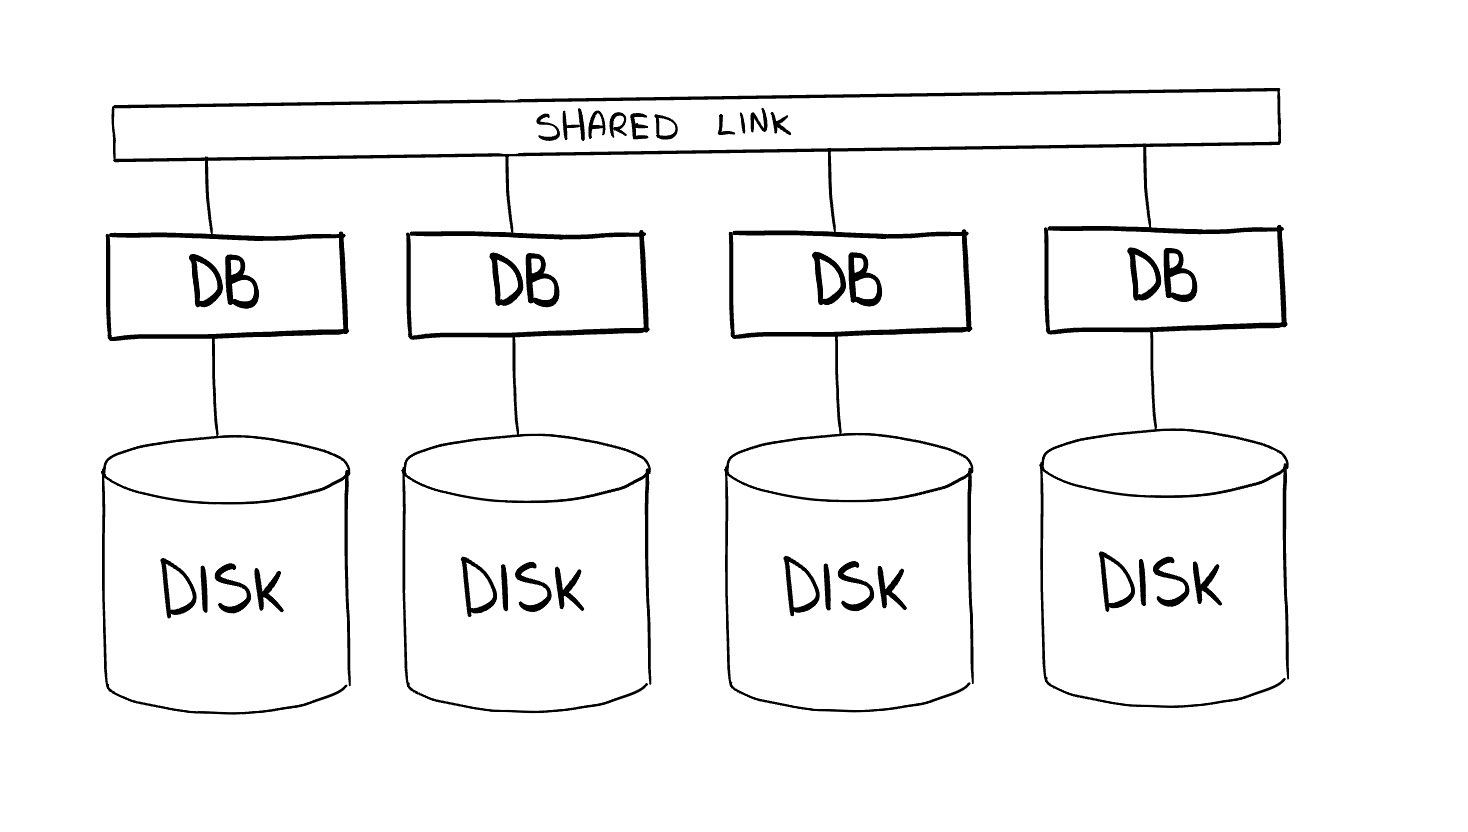
\includegraphics[width=0.5\textwidth]{img/SharedNothing.jpg}
      \caption{Architettura shared-nothing}
      \label{fig:sharedNothing}
\end{figure}
Esistono diverse architetture di DBMS distribuiti alcune delle quali sono
riportate in figura \ref{fig:DBMS_distributed_architecture}.
\begin{figure}[!ht]
      \centering
      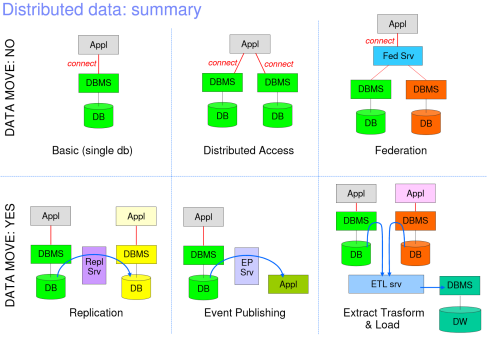
\includegraphics[width=0.5\textwidth]{./img/DBMS/DBMS_distributed_architecture.png}
      \caption{Architetture di DBMS distribuiti}
      \label{fig:DBMS_distributed_architecture}
\end{figure}

Non avendo il concetto di eterogeneità si mantiene lo stesso schema di un DBMS
centralizzato, distribuendo i dati. Questo comporta la necessità di aggiungere
uno schema logico locale tra lo schema logico e quello fisico. Non si avrà più
un solo schema logico e un unico schema fisico, ma tanti schemi logici locali e
fisici locali (ad ogni logico corrisponde un fisico).

I vari schemi logici locali si interfacciano con uno schema logico globale,
tali schemi non sono altro che delle viste dello schema logico globale. Questa
organizzazione tra schemi logici locali e schema logico globale è la cosiddetta
organizzazione \textbf{LAV} (Local As View). L'applicazione interroga
lo schema logico globale e successivamente verranno mappate le query distribuite 
sugli schemi logici locali.

% TODO: inserisci immagine dello schema logico

Per la gestione delle query distribuite serve una cooperazione o un'orchestrazione
dei singoli DBMS che fanno parte della federazione, soprattutto per quanto riguarda
il query processing e la gestione delle transazioni. Più precisamente si può avere
una gestione centralizzata (che può essere gerarchica) oppure distribuita con
un'assegnazione statica o dinamica dei ruoli. La scelta delle modalità
si effettuerà attraverso dei protocolli.

Nella fase di \textbf{progettazione} di un \textbf{DDBMS} si hanno delle
differenze rispetto alla progettazione di un DBMS centralizzato. Si hanno cinque fasi:
\begin{enumerate}
      \item Analisi dei requisiti
      \item Progettazione concettuale
      \item Progettazione della distribuzione, per capire dove mettere i dati
      \item Progettazione logica locale per ciascun nodo, che traduce dallo schema
            concettuale globale allo schema logico locale solo alcuni concetti
      \item Progettazione fisica locale per ciascun nodo
\end{enumerate}
Per quanto riguarda DBMS DEA (distribuiti eterogenei e autonomi) dal momento che
sono composti da DBMS eterogenei allora si introduce il concetto di \textbf{portabilità},
ovvero la capacità di eseguire le stesse applicazioni DB (SW per ottenere i dati
dal database) in ambienti runtime diversi. Questo viene facilitato dagli standard
dei linguaggi di query del database.

Inoltre, viene aggiunto anche il concetto di \textbf{interoperabilità}, ovvero
la capacità di eseguire applicazioni che coinvolgono contemporaneamente sistemi
diversi ed eterogenei. A tal fine sono si introducono dei \textbf{middleware},
tra cui \textbf{ODBC} che si occupa dell'accesso a dati di diversi vendor.
\textbf{ODBC}, a livello architetturale, si pone sopra il DBMS e da un'immagine
indipendente da ciò che c'è sotto, trasformando tutto in una sorta di SQL standard.
Si hanno anche dei protocolli, come \textbf{X-Open Distributed Transaction Processing}
(DTP) che consentono di eseguire delle transazioni secondo
una logica diversa. Questo protocollo stabilisce una serie di API che vengono
implementate da ogni singolo DBMS per offrire una connettività standard.

Il protocollo funziona sia se si ha che fare con omogeneità che con eterogeneità
dei DDBMS.

% ! da spostare
Si hanno altri approcci:
\begin{itemize}
      \item \textbf{Basi dati parallele}, con incremento delle prestazione
            mediante parallelismo sia di storage devices che di processore
            (scalabilità orizzontale).
      \item \textbf{Basi dati replicate} dove si ha la replicazione della stessa
            informazione su diversi server per motivi di performance. Importanti
            per i temi della consistenza e della sicurezza
      \item \textbf{Data warehouses}, ovvero DBMS centralizzati, risultato
            dell'integrazione di fonti eterogenee, dedicati nel dettaglio alla
            gestione di dati per il supporto alle decisioni. Prevede la
            cristallizzazione dei dati, acquisiti da varie sorgenti, creando un
            nuovo schema con la memorizzazione dei dati in formato nuovo
            (solitamente relazionale). Non usa un approccio LAV.
\end{itemize}
\subsection{Vantaggi dei DDBMS}
I \textbf{DDBMS} hanno notevoli \textbf{vantaggi}:
\begin{itemize}
      \item \textbf{Località}: i dati sono vicino alle applicazioni che li
            utilizzano più frequentemente. Questo riduce i tempi per l'esecuzione
            delle operazioni. Il paradigma è spostare i dati verso le
            applicazioni, le partizioni dei dati corrispondono spesso a delle
            partizioni naturali delle applicazioni e degli utenti. Le
            distribuzioni dei dati spesso sono flessibili: è possibile spostare un
            intera tabella così come è possibile spostarne solo un sottoinsieme
            o replicarla.
      \item \textbf{Modularità} le modifiche alle applicazioni e ai dati possono
            essere effettuate a basso costo. Si ha una distribuzione dei dati
            incrementale e progressiva, infatti la configurazione si adatta alle
            esigenze delle applicazioni.
      \item \textbf{Resistenza ai guasti}: grazie alla replicazione dei dati si ha
            ridondanza (fail soft). Ovviamente la ridondanza funziona in rete quindi
            si introduce fragilità per la comunicazione in rete.
      \item \textbf{Prestazioni ed Efficienza}: distribuendo un database su più
            nodi, ogni nodo gestisce un DB di dimensioni ridotte. Questo
            significa che i singoli DB sono più facili da gestire e ottimizzare
            localmente e, in particolare, ogni nodo può adottare delle
            ottimizzazioni personalizzate. Il carico inoltre viene distribuito
            sui nodi che permette di avere parallelismi tra le transazioni che fanno
            parte della stessa transazione distribuita.
            Tutto ciò però richiede chiaramente un coordinamento tra i
            nodi e aumenta il traffico di rete che può rivelarsi un collo di
            bottiglia per le prestazioni.
\end{itemize}
\subsection{Differenze rispetto ai DBMS}
Si ha un \textbf{indipendenza locale e cooperazione tra server}, ogni server
mantiene ha la sua applicazione, si hanno interazioni tra i vari server per la
loro cooperazione, la cooperazione può avvenire per gestire due cose:
\begin{itemize}
      \item \textbf{interrogazioni}: sia query provenienti dalle applicazioni e
            i risultati provenienti dal server
      \item \textbf{transazioni}: richieste di transazioni dalle applicazioni  e
            dati di controllo per il coordinamento dello stato delle transazioni.
\end{itemize}
Il problema è legato all'ottimizzazione, la quale è limitata per via della rete. 
L'obiettivo sarà quello di distribuire i dati per avere più transazioni possibili 
in locale in modo da limitare lo scambio di messaggi tra i vari server.

Si hanno anche le seguenti funzionalità specifiche:
\begin{itemize}
      \item \textbf{Trasmissione} di query, transizioni, frammenti di db e dati
            di controllo tra i nodi.
      \item \textbf{Frammentazione, replicazione e trasparenza} fattori legati
            alla natura distribuita dei dati.
      \item un query processor e un query plan per la previsione di una
            strategia globale accanto a strategie per le query locali. Si gestisce
            il passaggio tra schema logico globale e quelli locali. Chi esegue
            la query lo fa senza pensare alla frammentazione dei dati
      \item \textbf{Controllo di concorrenza} tramite algoritmi distribuiti, fondamentale
            per gli accessi in scrittura.
      \item \textbf{Strategie di recovery} e \textbf{gestione dei guasti}, sia
            in merito alla rete, sia all'hardware stesso.
\end{itemize}
\subsection{Frammentazione}
\begin{definizione}[\textbf{Frammentazione}]
      Si definisce \textbf{frammentazione} come la possibilità di allocare porzioni
      diverse del database su nodi diversi.
\end{definizione}
Esistono due tipi di frammentazione:
\begin{itemize}
      \item \textbf{orizzontale}: si prende una tabella e la si
            frammenta in base alle righe. Si mantiene inalterato lo schema in
            quanto si ottengono solo delle tabelle più piccole. Per spezzare si
            usa una select che selezioni ogni volta un certo blocco di tabella.
            (Ex: vengono separati i dottori nati a Milano da quelli nati a Napoli,
            alla fine si effettua la union per ricostruire la tabella originale)
      \item \textbf{verticale}: si prende una tabella e la si frammenta
            in base alle colonne. In ogni nuova tabella però la prima colonna
            deve essere uguale alla prima della tabella originale (ovvero dove si
            ha la chiave primaria), questo per garantire che si possa ricomporre
            la tabella originale con operazioni di join e garantire la
            trasparenza. Anche in questo caso uso una select che selezioni ogni
            volta un certo numero di colonne da mettere nella nuova tabella.
\end{itemize}
Quando si usa la frammentazione bisogna garantire le seguenti regole:
\begin{itemize}
      \item \textbf{Completezza}: ogni record della relazione R di partenza
            deve poter essere ritrovato in almeno uno dei frammenti.
      \item \textbf{Ricostruibilità}: la relazione R di partenza deve poter essere
            ricostruita senza perdita di informazione a partire dai frammenti.
      \item \textbf{Disgiunzione}: ogni record della relazione R deve essere
            rappresentato in uno solo dei frammenti.
      \item \textbf{Replicazione}: l'opposto della disgiunzione.
\end{itemize}
\begin{esempio}[\textbf{Esercizio 1, esercitazione 1}]
      Esempio esercitazione frammentazione delle tabelle nelle posizioni geografiche.
      La tabella \textbf{Production} verrà frammentata orizzontalmente in questo modo:
      \begin{equation*}
            Poduction1=\sigma_{PartType=CPU}(Production)
      \end{equation*}
      \begin{equation*}
            Poduction2=\sigma_{PartType=Keyboard}(Production)
      \end{equation*}
      \begin{equation*}
            Poduction3=\sigma_{PartType=Screen}(Production)
      \end{equation*}
      \begin{equation*}
            Poduction4=\sigma_{PartType=Pipe}(Production)
      \end{equation*}
      La tabella \textbf{Pickup} verrà frammentata orizzontalmente in questo modo:
      \begin{equation*}
            Pickup1=\pi_{SN, Lot, Client,SalesPerson, Amount}(\sigma_{PartType=CPU}(Production)\triangleright\triangleleft_{Pickup.SN=Production.SN}(Pickup))
      \end{equation*}
      \begin{equation*}
            Pickup2=\pi_{SN, Lot, Client,SalesPerson, Amount}(\sigma_{PartType=Keyboard}(Production)\triangleright\triangleleft_{Pickup.SN=Production.SN}(Pickup))
      \end{equation*}
      \begin{equation*}
            Pickup3=\pi_{SN, Lot, Client,SalesPerson, Amount}(\sigma_{PartType=Screen}(Production)\triangleright\triangleleft_{Pickup.SN=Production.SN}(Pickup))
      \end{equation*}
      \begin{equation*}
            Pickup4=\pi_{SN, Lot, Client,SalesPerson, Amount}(\sigma_{PartType=Pipe}(Production)\triangleright\triangleleft_{Pickup.SN=Production.SN}(Pickup))
      \end{equation*}
      Per frammentare \textbf{SalesPerson} si può frammentare in questo modo:
      \begin{equation*}
            SalesPerson1=\sigma_{City=SanJose}(SalesPerson)
      \end{equation*}
      \begin{equation*}
            SalesPerson2=\sigma_{City=Zurich \lor City=Dublin}(SalesPerson)
      \end{equation*}
      \begin{equation*}
            SalesPerson3=\sigma_{City=Taiwan}(SalesPerson)
      \end{equation*}
      Per frammentare \textbf{Client} si può frammentare in questo modo:
      \begin{equation*}
            Client1=\sigma_{City=SanJose}(Client)
      \end{equation*}
      \begin{equation*}
            Client2=\sigma_{City=Zurich \lor City=Dublin}(Client)
      \end{equation*}
      \begin{equation*}
            Client3=\sigma_{City=Taiwan}(Client)
      \end{equation*}
      Le tabelle appena calcolate verranno distribuite nel seguente modo:
      \begin{itemize}
            \item \textbf{San Josè}: Production1, Pickup1, Client1 e Sales1 
            \item \textbf{Zurich}: Production2, Pickup2, Client2 e Sales2 
            \item \textbf{Taiwan}: Production3, Pickup3, Client3 e Sales3
            \item \textbf{Dublin}: Production4 
      \end{itemize}
\end{esempio}
\subsection{Replicazione}
\begin{definizione}[\textbf{Replicazione}]
      Si definisce \textbf{replicazione} come la possibilità di allocare stesse
      porzioni del database su nodi diversi.
\end{definizione}
Si hanno diversi aspetti positivi per l'accesso in lettura, come il miglioramento
delle prestazioni in quanto consente la coesistenza di applicazioni con requisiti
operazionali diversi sugli stessi dati e aumenta la località dei dati usati da
ogni applicazioni. Nel momento in cui si ha l'accesso in scrittura si hanno però
diversi aspetti negativi. Si hanno diverse complicazioni architetturali, tra cui
la gestione della transazioni e l'update di copie multiple, che devono essere
tutte aggiornate. Inoltre bisogna studiare dal punto di vista progettuale cosa
replicare, quanto replicare, dove allocare le copie e le politiche per gestirle.

In merito all'allocazione studiamo anche gli schemi di allocazione. Ogni
frammento può essere allocato su un nodo diverso. Lo schema globale quindi
è solo virtuale e lo schema di allocazione definisce il mapping tra un frammento
e un nodo. Si ha quindi una tabella, un catalogo, che ci da informazioni sul
partizionamento, associando ogni frammento al nodo in cui è allocato.
\subsection{Trasparenza}
\begin{definizione}[\textbf{Trasparenza}]
      Si definisce \textbf{trasparenza} come la possibilità per l'applicazione di
      accedere ai dati senza sapere dove sono allocati.
\end{definizione}
Con la trasparenza si ha la separazione della semantica di alto livello dalle
modalità di frammentazione e allocazione. Si separa quindi la logica applicativa
dalla logica dei dati ma per farlo serve uno strato software che gestisca la
traduzione dallo schema unico ai sottoschemi, comportando un aumento di
complessità del sistema e una perdita di prestazioni.
Le applicazioni (transazioni, interrogazioni) non devono essere modificate a
seguito di cambiamenti nella definizione e organizzazione dei dati e si hanno
due tipi di trasparenza, che si applicano agli schemi ANSI-SPARC nel
modello distribuito:
\begin{enumerate}
      \item \textbf{Trasparenza logica} (o indipendenza logica), ovvero
            indipendenza dell'applicazione da modifiche dello schema logico.
            Un'applicazione che usa un frammento non viene modificata se vengono
            modificati altri frammenti.
      \item \textbf{Trasparenza fisica} (o indipendenza fisica), ovvero
            indipendenza dell'applicazione da modifiche dello schema fisico
\end{enumerate}

Frammentazione e allocazione sono tra lo schema logico globale e ogni schema
logico locale. Si hanno quindi tre livelli di trasparenza:
\begin{itemize}
      % TODO: immagini sull'effetto della trasparenza nelle  query
      \item \textbf{Trasparenza di frammentazione}, che permette di ignorare
            l'esistenza dei frammenti ed è lo scenario migliore per la
            programmazione applicativa. Il sistema si occupa di convertire query
            globali in locali e relazioni in sotto-relazioni. La scomposizione
            delle query per ogni sotto-relazione è detta query rewriting.
      \item \textbf{Trasparenza di replicazione/allocazione}, dove l'applicazione
            è consapevole dei frammenti ma non dei nodi in cui si trovano. In questo
            caso la query è già spezzata in quanto si sa di avere a che fare con un
            sistema frammentato.
      \item \textbf{Trasparenza di linguaggio}, dove l'applicazione specifica
            sia i frammenti che i nodi, nodi che possono offrire interfacce che
            non sono SQL standard. Tuttavia l'applicazione sarà scritta in SQL
            standard a prescindere dai linguaggi locali dei nodi. Le query
            vengono quindi tradotte ottimizzatone di query. Questo è il livello
            di trasparenza più basso.
\end{itemize}
\begin{esempio} [\textbf{esercizio 1, esertcitazione 1}]
      Eseguiamo le seguenti query:
      \begin{itemize}
            \item prima query:
            \begin{itemize}
                  \item \textbf{trasparenza di frammentazione} (specifichiamo solo la tabella logica): \texttt{SELECT quantity FROM Production WHERE SerialNumber = 77y6878}
                  \item \textbf{trasparenza di replicazione/allocazione} (specifichiamo il frammento al quale effettuare la richiesta): \texttt{SELECT quantity FROM Production1 WHERE SerialNumber = 77y6878 UNION SELECT quantity FROM Production2 WHERE SerialNumber = 77y6878 UNION SELECT quantity FROM Production3 WHERE SerialNumber = 77y6878  }
                  \item \textbf{trasparenza di linguaggio} (specifichiamo il nodo al quale effettuare la richiesta): \texttt{SELECT quantity FROM Production1@company.SanJose.com WHERE SerialNumber = 77y6878 UNION SELECT quantity FROM Production2@company.Taiwan.com WHERE SerialNumber = 77y6878 UNION SELECT quantity FROM Production3@company.Zurich.com WHERE SerialNumber = 77y6878  }
            \end{itemize}
            \item seconda query:
            \begin{itemize}
                  \item \textbf{trasparenza di frammentazione}: 
                  \item \textbf{trasparenza di replicazione/allocazione}: \texttt{SELECT client FROM Pickup3 as P JOIN SalesPerson as S ON P.SalesPerson = S.SalesID WHERE S.Name = "Brown"}
                  \item \textbf{trasparenza di linguaggio}: \texttt{SELECT client FROM Pickup3@company.Taiwan.com as P JOIN SalesPerson@company.Taiwan.com as S ON P.SalesPerson = S.SalesID WHERE S.Name = "Brown"}
            \end{itemize}
            \item terza query:
            \begin{itemize}
                  \item \textbf{trasparenza di frammentazione}:  \texttt{SELECT machine FROM Produciton as P JOIN Pickup as PU ON P.SN = PU.SN JOIN Client ON Client.id=client WHERE S.Name = "Brown" AND parttype="Keyboard"}
                  \item \textbf{trasparenza di replicazione/allocazione}:  \texttt{SELECT machine FROM Produciton2 as P JOIN Pickup2 as PU ON P.SN = PU.SN JOIN Client2 ON Client.id=client WHERE S.Name = "Brown" AND parttype="Keyboard"}
                  \item \textbf{trasparenza di linguaggio}:  \texttt{SELECT machine FROM Produciton2@company.com as P JOIN Pickup2@company.com as PU ON P.SN = PU.SN JOIN Client2@company.com ON Client.id=client WHERE S.Name = "Brown" AND parttype="Keyboard"}
            \end{itemize}
            \item quarta query:
            \begin{itemize}
                  \item \textbf{trasparenza di frammentazione}:  \texttt{UPDATE FROM Client SET address="k3$\dots$" AND City="Taiwa" WHERE name="$\dots$"}
                  \item \textbf{trasparenza di replicazione/allocazione}:  prima si inserisce il nuovo record
                  \texttt{INSERT INTO Client3 (Name, City,Address) VALUES ("Brown", "Taiwan", "43$\dots$")}\\ successivamente cancelliamo il cliente dalla vecchia tabella
                  \texttt{DELETE FROM Client1 WHERE name="Brown"}
            \end{itemize}
            \item quinta query:
            \begin{itemize}
                  \item \textbf{trasparenza di frammentazione}:  \texttt{SELECT city, SUM(amount) FROM Pickup JOIN Client ON Client=ClientID GROUP BY city}
                  \item \textbf{trasparenza di replicazione/allocazione}: creiamo prima
                  le view delle tabelle non frammentate
                  \texttt{CREATE VIEW Client UNION Client1 UNION Client2 UNION Client3} \\
                  \texttt{CREATE VIEW Pickup UNION Pickup1 UNION Pickup2 UNION Pickup3} \\ 
                  \texttt{SELECT city, SUM(amount) FROM Pickup JOIN Client ON Client=ClientID GROUP BY city}
            \end{itemize}
      \end{itemize}
\end{esempio}
\section{Gestione delle query distribuite}
In un DBMS distribuito, a differenza dei DBMS centralizzati, le query vengono ottimizzate
in modo diverso. In particolare, si hanno le seguenti fasi:
\begin{itemize}
      \item \textbf{Query decomposition}: la query distribuita viene decomposta in
            sotto-query che possono essere eseguite in modo indipendente. Questa
            fase tiene conto dello schema logico globale e non considera la
            distribuzione dei dati. Usa delle tecniche di ottimizzazione algebrica
            come quelle usate nei DBMS centralizzati.
            In output a questa fase si ha un \textbf{query tree globale} che non tiene
            conto dei costi di comunicazione.
      \item \textbf{Data Location}: in questa fase si considera la distribuzione
            dei frammenti. Si ottimizzano le operazioni rispetto alla
            frammentazione utilizzando tecniche di riduzione. In output si ha una
            \textbf{query efficiente sui frammenti} ma non ottimizzata.
      \item \textbf{Global optimization}: in questa fase si ottimizza la query
            rispetto ai costi di comunicazione, aggiungendo agli operatori
            algebrici quelli per la comunicazione. L'obiettivo è quello di
            trovare il piano di esecuzione che minimizza il costo totale, ovvero
            l'ordine migliore delle operazioni nella query fragment. Le
            decisioni più importanti riguardano le operazioni di join perché
            non si possono trasferire gli indici e quindi è l'operazione più lenta
            (scelta se usare un join o semi-join) (Si ottimizza il costo di comunicazione).
      \item \textbf{Local optimization}: in questa fase si ottimizza il piano di
            esecuzione per ogni singolo nodo (si ottimizza indipendentemente il
            query fragment usando le ottimizzazioni centralizzate).
\end{itemize}
Gli obiettivi dell'ottimizzazione sono ridurre il costo totale, ovvero la somma
dei costi di operazioni locali come input e output, e il costo di comunicazione.
Oltre a ciò, si vuole ridurre il response time, ovvero la somma dei costi tenendo
conto del parallelismo.
\begin{figure}[!ht]
      \centering
      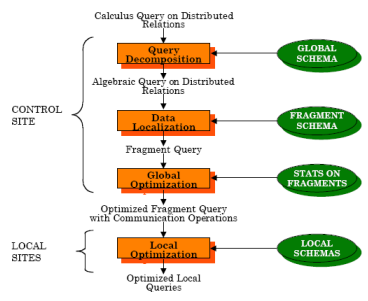
\includegraphics[width=0.5\textwidth]{./img/DDBMS/query.png}
      \caption{Fasi dell'ottimizzazione delle query distribuite}
      \label{fig:queryOptimization}
\end{figure}
% TODO: aggiungere l'esempio nelle slide

Il costo principale nelle basi di dati è il \textbf{costo totale} che è dipendente
dai \textbf{costi delle operazioni} (I/O e CPU) e dal costo di \textbf{costo di comunicazione}.
\begin{center}
      \text{costo totale} = \textbf{costo operazioni} + \textbf{costo di comunicazione}
\end{center}
Se si sommano tutti i costi di tutte le operazioni eseguite nella query distribuita,
tenendo conto del parallelismo, si ottiene il \textbf{response time}.

Nel caso distribuito il \textbf{costo di comunicazione} è quello più significativo rispetto
ai \textbf{costi delle operazioni}. Per calcolare i costi di comunicazione si
può seguire la seguente formula.
\begin{equation*}
      \text{Costo comunicazione} = \text{C\_{MSG}} \cdot \#\ msgs  + \text{C\_{TR}} \cdot \#bytes
\end{equation*}
dove:
\begin{itemize}
      \item \textbf{$C\_{MSG}$} è il costo di trasmissione di un messaggio
      \item \textbf{$C_{TR}$} è il costo di trasmissione fisso di un byte
            dipendente dalla topologia
      \item \textbf{$\#\ msgs$} è il numero di messaggi
      \item \textbf{$\#bytes$} è il numero di byte
\end{itemize}
Per calcolare il \textbf{tempo di risposta} (response time), a differenza del
costo totale, i costi delle operazioni in parallelo non si sommano,
ottenendo la seguente formula:
\begin{equation*}
      \text{Tempo di risposta} = C\_{MSG} \cdot seq\_\#msgs + C_{TR} \cdot seq\_\#bytes
\end{equation*}
dove $seq\_\#msgs$ è il massimo numero di messaggi che devono essere comunicati
in modo sequenziale.

Naturalmente, il costo più importante deve essere valutato in base a alla
situazione in cui mi trovo. Chiaramente se si lavora in una grande rete
geografica, il costo di comunicazione sarà molto più alto rispetto al costo di
esecuzione locale. Viceversa nelle reti locali, il costo di comunicazione sarà
molto più basso rispetto al costo di esecuzione locale. Ovviamente possiamo calcolare
il costo totale assegnando dei pesi ai singoli costi.

Possiamo essere interessati a:
\begin{itemize}
      \item \textbf{Minimizzazione tempo di risposta}: più parallelismo può portare ad
            aumento del costo totale (maggiore numero di trasmissioni e
            processing locale)
      \item \textbf{Minimizzazione costo totale}: somma dei costi senza tener conto del
            parallelismo: utilizza meglio le risorse e aumento del throughput (con
            peggioramento del response time in generale)
\end{itemize}
\subsection{Operazione di join}
Dato che nei join quando si trasferiscono i dati non è possibile passare gli indici,
le operazioni di join sono quelle più costose dal punto di vista computazionale.
Per questo motivo, l'operazione di \textbf{semijoin} può essere in alcune circostanze
un'alternativa più efficiente rispetto al join.
\begin{definizione}[\textbf{Semijoin}]
      Dati due insiemi $R$ e $S$, il semijoin di $R$ e $S$ è definito come:
      \begin{equation*}
            R \text{semijoin}_A S \equiv \pi_{R^\ast}(R \, \text{join}_A \, S)
      \end{equation*}
      dove $R^\ast$ è l'insieme delle colonne di $R$. Il semijoin è la proiezione
      sugli attributi di $R$ del join di $R$ e $S$.
\end{definizione}
\begin{nota}
      Il semijoin non è commutativo.
\end{nota}
Chiaramente l'uso del semi - join è conveniente se il costo del suo calcolo e
del trasferimento del risultato sono inferiori al costo di trasferimento
dell'intera relazione del costo del join intero.

In generale, l'uso del semijoin è più conveniente se il costo del suo calcolo e
del trasferimento del risultato è inferiore al consto del trasferimento
dell'intera relazione e del costo del join intero.
\section{Controllo della concorrenza}
Fino a questo momento abbiamo considerato le interrogazioni più semplici. Vogliamo
ora analizzare la gestione delle scritture sui database distribuiti. In particolare,
possiamo classificare le transazioni in due categorie:
\begin{itemize}
      \item \textbf{Dirette a un unico server remoto}: in questo caso il controllo
            della concorrenza è simile a quello dei DBMS centralizzati. Dobbiamo
            distinguere tra due tipi di transazioni:
            \begin{itemize}
                  \item \textbf{Remote request}: ovvero transazioni di sola lettura
                  \item \textbf{Remote transaction}: ovvero transazioni di lettura
                        e scrittura.
            \end{itemize}
      \item \textbf{Dirette a un numero arbitrario di server}: in questo caso il
            controllo della concorrenza è più complesso. In questo caso la
            classificazione si divide in:
            \begin{itemize}
                  \item \textbf{Distributed requests}: operazioni read - only
                        arbitrarie nelle quali ogni singola operazione SQL si può
                        riferire a qualunque insieme dei server. Richiede un
                        ottimizzatore distribuito.
                  \item \textbf{Distributed transactions}: numero arbitrario di
                        operazioni SQL, ogni operazione è diretta ad un unico
                        server. Le transazione possono modificare più di un
                        database. Richiede un protocollo transazionale di
                        coordinamento distribuito (two - phase commit).
            \end{itemize}
\end{itemize}
La \textbf{distribuzione} non ha conseguenze su \textbf{consistenza} e \textbf{durabilità}
in quanto la consistenza non dipende dalla distribuzione poiché i vincoli descrivono
solo proprietà logiche dello schema. Mentre, la durabilità è garantita localmente
da ogni sistema.

È invece necessario rivedere alcuni componenti dell'architettura in merito a
\textbf{isolamento} tramite concurrency control e ad \textbf{atomicità} tramite
reliability control e recovery manager.

L'idea alla base del controllo della concorrenza è che ogni transizione $t_i$
possa essere suddivisa in $t_{ij}$ transazioni che saranno eseguite sul nodo $j$.
Ogni sotto-transazione viene schedulata in modo indipendente dai server di
ciascun nodo. La schedule globale dipende quindi dalle schedules locali su ogni nodo.

In questo modo lo schedule globale andrà a dipendere dallo schedule locale di
ciascun nodo. Inoltre in questo caso, seppur localmente le transazioni sembrino
serializzabili, si crea la possibilità di avere conflitto a livello globale.

Una prima soluzione potrebbe essere la serializzazione locale delle sotto-transazioni,
ma questo non assicura la serializzabilità globale.

Nel caso di database \textbf{non è replicato} e ogni \textbf{schedule locale} è
\textbf{serializzabile} allora lo  \textbf{schedule globale} è \textbf{serializzabile}
se gli ordini di serializzazione sono gli stessi per tutti i nodi, ovvero se il
flusso delle transazioni è lo stesso per tutti i nodi.

Quando si aggiunge la  \textbf{replicazione dei dati} le cose cambiano. Nello
specifico possiamo violare la \textbf{mutua consistenza dei database locali} per
la quale tutte le copie devono avere lo stesso valore al termine della transazione.
Abbiamo quindi bisogno di un \textbf{protocollo di controllo delle repliche}.
\subsection{ROWA}
Un protocollo è il \textbf{ROWA} (\textbf{Read Once Write All}). Questo
protocollo mappa le operazioni di lettura su una qualunque delle copie, mentre
le operazioni di scrittura vengono mappate su tutte le copie. Di fatto, finché
non sono accertate tutte le write su tutte le copie, la transazione non continua.

Questo protocollo garantisce la \textbf{consistenza dei dati}, ma a scapito
chiaramente delle performance. Questa condizione può essere rilassata con dei
protocolli asincroni più efficienti.
\subsection{Two Phase Locking}
Nella progettazione della base di dati bisogna considerare diverse informazioni:
\begin{itemize}
      \item Topologia della rappresentazione.
      \item Tipologie di query distribuite.
      \item Stime o statistiche su query distribuite.
\end{itemize}
In aggiunta dobbiamo considerare i problemi di scrittura e quindi problemi di
concorrenza. Dobbiamo costruire una serie di protocolli che ci permettono di
risolvere questi problemi, nel sistema centralizzato un metodo è quello di usare
2PL, il quale sfrutta i lock (accesso esclusivo) sulle risorse (tabelle, blocchi
di pagina o righe) per eseguire le transazioni.

Vediamo ora come possiamo risolvere questo problema nel caso \textbf{distribuito}. Sul
\textbf{singolo nodo} le transazioni verranno gestite come nel caso \textbf{centralizzato}. Questo
però non risolve i problemi di deadlock distribuiti. Per risolvere questo problema
bisogna avere una \textbf{vista globale del sistema}, in aggiunta tutto si complica
aggiungendo le repliche.

Con l'aggiunta di quest'ultime si introduce il problema sull'\textbf{atomicità}, perché
bisogna assicurarsi che una scrittura venga replicata su tutti i nodi e che sia
fatta in modo efficiente. Una soluzione a questo problema è il protocollo \textbf{ROWA},
il quale consiste nello scrivere su tutte le repliche e poi segnalano quando
hanno finito, in questo modo posso leggere da qualsiasi nodo. Questo approccio
comporta rallentamenti dal momento che le repliche sono dislocate geograficamente.

Si può estendere \textbf{2PL al caso distribuito} introducendo un coordinatore delle
transaction centrale e un lock manager per ogni nodo. Uno di questi lock manager
viene eletto come coordinatore e si occupa di gestire i lock tra i vari nodi.

La strategia in questo caso è quella che il Transaction Manager (TM) lancia la
transazione e utilizza un lock manager centrale che gestisce i lock tra tutti i
nodi. Il lock manager centrale la esegue utilizzando 2 phase locking. A questo
punto il transaction manager comunica ai data processor di eseguire le operazioni.
Una volta che il data processor ha finito, comunica al lock manager centrale che
ha finito e il lock manager centrale comunica al transaction manager che può fare
commit.

Questo approccio vuole simulare il comportamento di un sistema centrale su un
sistema distribuito. Questo introduce un problema a livello di comunicazione,
infatti il lock manager centrale diventa un collo di bottiglia, inoltre, si ha
single point of failure, casca il LM allora si rompe tutto.

Per mitigare il problema posso utilizzare un LM secondario che si attiva quando
il primo muore. Per mantenere allineato tutto si può usare ROWA il quale riduce
le performance. Per attivarlo si usano load balancer ma serve tempo quindi si
rischia sempre problemi.
\begin{figure}[!ht]
      \centering
      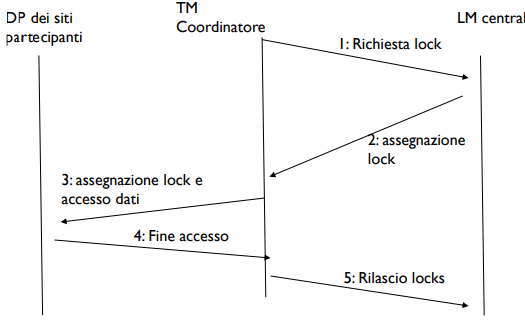
\includegraphics[width=.5\textwidth]{img/DDBMS/centralized_2PL.png}
      \caption{Esempio di 2PL centralizzato}
      \label{fig:2PL_centralizzato}
\end{figure}

Un'altra modalità per gestire i locking distribuiti è \textbf{primary copy 2PL}.
In questa strategia, per ogni risorsa viene individuata una \textit{copia primaria}
che viene selezionata prima dei lock. Ogni nodo ha un suo lock manager attivo che
gestisce una partizione dei lock complessivi relativi alle risorse primarie
contenute nel suo nodo. Per ogni transazione il TM chiede al lock manager del nodo
dove si trova la risorsa primaria, il quale si occupa di gestire i lock.

In questo modo si riduce il single point of failure e si riduce il traffico
sulla rete. Inoltre, si riduce il tempo di risposta perché si riduce il numero
di messaggi. Questo approccio però non è perfetto, infatti, è necessario avere
una directory globale che mappa le risorse primarie con i nodi in modo da poter
sapere a chi chiedere il lock.
\subsection{Deadlock distribuiti}
I deadlock distribuiti sono più complessi da gestire rispetto a quelli centralizzati
perché non si ha una visione globale del sistema.

Per la gestione di questi è possibile utilizzare un algoritmo di rilevamento.
Prima di analizzare tale algoritmo vediamo quali sono i tipi di attesa che
si possono avere in un sistema distribuito:
\begin{itemize}
      \item \textbf{Attesa da remote procedure call}
      \item \textbf{Attesa da rilascio di risorsa}
\end{itemize}
La composizione dei due tipi di attesa può dare luogo a uno stato di deadlock
globale.
\begin{figure}[!ht]
      \centering
      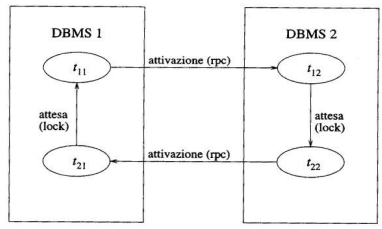
\includegraphics[width=.5\textwidth]{img/DDBMS/deadlock_distribuito.png}
      \caption{Esempio di deadlock distribuito}
      \label{fig:deadlock_distribuito}
\end{figure}

Possiamo caratterizzare le condizioni di attesa su ciascun nodo tramite delle
condizioni di precedenza usando al seguente notazione:
\begin{itemize}
      \item \textbf{$EXT_i$}: external, ovvero la chiamata da un nodo remoto $i$.
      \item $x < y$: ovvero $x$ attende il rilascio di una risorsa da $y$. Questo
            può anche essere remoto.
\end{itemize}
La sequenza di attesa generale al nodo è della forma:
\begin{equation*}
      EXT_i < x < y < EXT_j
\end{equation*}

\begin{nota}
      Prima di eseguire la transazione si effettua la richiesta di lock e solo 
      al suo termine rilascia il lock.
\end{nota}

Da osservatore esterno, riusciamo a vedere quando c'è un ciclo di attese e
quindi un deadlock globale, ma a livello di singolo nodo questo è più complicato.
La soluzione a questo problema avviene attivando periodicamente sui diversi nodi
delle procedure di rilevamento dei deadlock. Queste procedure si scambiano le
informazioni sui grafi di attesa locali e se si rileva un ciclo si attiva una
procedura di risoluzione del deadlock.

L'algoritmo di rilevamento dei \textbf{deadlock distribuiti} è composto come segue:
\begin{itemize}
      \item In ogni nodo, si integra il grafo locale con quello degli altri nodi
            che ho ricevuto.
      \item Si analizza il grafo in cerca di condizioni di attesa sul nodo e
            rileva i deadlock locali.
      \item Comunica le sequenze di attesa agli altri nodi. L'ordine di
            comunicazione va dal nodo più piccolo a quello più grande
\end{itemize}

È possibile ovviamente che lo stesso deadlock venga riscoperto più volte. Per
evitare ciò e rendere più efficiente l'algoritmo si inviano le sequenze di attesa
nei seguenti modi:
\begin{itemize}
      \item In avanti verso il nodo dove è attiva la sotto-transazione $t_i$
            attesa da $t_j$.
      \item Solamente quando $i > j$ dove $i$ e $j$ identificano i nodi.
\end{itemize}

L'ordine dei nodi si decide a priori durante la progettazione del sistema distribuito.

% TODO: aggiungere esempio
\section{Recovery Management}
In un sistema distribuito i problemi riguardanti l'atomicità possono essere
suddivisi in:
\begin{itemize}
      \item \textbf{Problemi locali}: ogni singolo nodo può avere problemi, come ad
            esempio rottura disco, bug nel SW.
      \item \textbf{Problemi globali}: come la perdita di messaggi oppure legati al
            partizionamento della rete, ovvero quando due o più porzioni della
            rete non riescono a vedersi per vari motivi e considerano l'altra
            parte morta.
\end{itemize}
La gestione dei problemi di partizionamento può essere fatta con una soluzione
centralizzata in cui un nodo decide se la transazione distribuita deve essere
conclusa con un commit o con un abort (orchestrato) (2PC).

I server sono chiamati \textbf{Resource Manager} (RM) ed il coordinatore è
chiamato \textbf{Transaction Manager} (TM). Il protocollo di coordinamento
distribuito è chiamato \textbf{Two Phase Commit} (2PC) e si basa sullo scambio
di messaggi tra TM e RM.

In assenza di guasti, il funzionamento del protocollo è il seguente:
\begin{itemize}
      \item \textbf{Fase 1}: il TM chiede ai RM come intendono terminare la
            transazione. Ogni RM risponde autonomamente con un messaggio in cui
            comunica se è un commit locale o un abort.
      \item \textbf{Fase 2}: il TM prende una decisione comune, se un solo RM
            risponde con un abort, allora la decisione è abort, altrimenti è
            commit. A questo punto il TM comunica la decisione ai RM.
\end{itemize}
La gestione di tutte le operazioni avviene tramite i log, in particolare, il TM
scrive nel suo file di log prima di prendere la decisione,
in modo da poter ripristinare lo stato del sistema in caso di guasto. Lo stesso
viene fatto dai vari RM.
\begin{figure}[!ht]
      \centering
      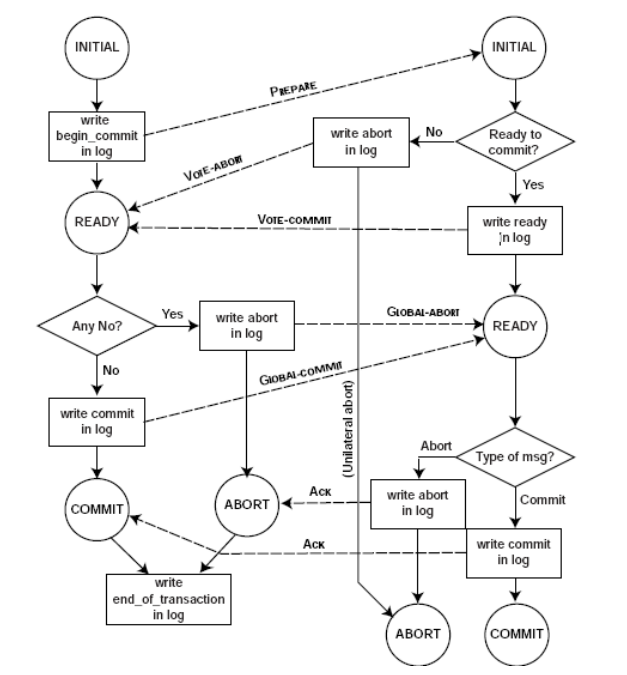
\includegraphics[width=.5\textwidth]{img/DDBMS/2PC.png}
      \caption{Fasi del protocollo 2PC}
      \label{fig:2PC}
\end{figure}

Nei log compaiono due tipi di record:
\begin{itemize}
      \item \textbf{Record di transazione}: contiene informazioni sulle operazioni
            effettuate.
      \item \textbf{Record di sistema}: checkpoint e dump.
\end{itemize}

Per il \textbf{transaction manager} i record di sistema sono:
\begin{itemize}
      \item \textbf{Record di Prepare} contenente l'identità di tutti i RM (nodi + transazioni).
      \item \textbf{Global Commit o Abort} che indica come è finita la transazione. La
            decisione diventa esecutiva quando il TM scrive nel proprio log
            questo record.
      \item \textbf{Complete} per indicare che la transazione è completata.
\end{itemize}
Per i \textbf{Resource Manager} i record di sistema sono:
\begin{itemize}
      \item \textbf{Ready Record} indica la disponibilità irrevocabile del RM a
            partecipare alla fase di commit e contiene l'identificatore del TM.
      \item \textbf{Not Ready} indica la indisponibilità del RM al commit.
\end{itemize}

Essendo in un modo distribuito le comunicazioni potrebbero non arrivare, perciò
si utilizzano dei \textbf{timeout}.
Nella \textbf{prima fase} TM effettua la richiesta di disponibilità con un timeout
per chiedere ai RM se sono disponibili. Se il tempo del timeout termina senza
risposta, la mancata risposta si considera come non disponibile
o abort. Inoltre, si utilizza un timeout anche per la \textbf{seconda fase} con lo
scopo di attendere gli ACK dei RM sul commit, se TM non riceve la conferma allora
continua a mandare richieste di conferme fino a quando tutti rispondono.

Questo algoritmo può essere ottimizzato modificando la comunicazione, la quale
può avvenire dal TM in broadcast oppure TM comunica col primo RM e il primo RM
scrive agli altri. In questo modo l'ultimo permette di non avere la seconda fase
nel TM.

Fino a questo momento abbiamo studiato il caso ottimale, ovvero quello in assenza
di guasti. Nella realtà i guasti possono capitare in vari momenti, come ad esempio:
\begin{itemize}
      \item \textbf{Write begin commit}: se uno degli RM non risponde entro il tempo
            prestabilito viene fatto l'abort della transazione.
      \item Se nella fase in cui il TM deve ricevere la conferma qualche RM non
            risponde, allora il transaction manager invia nuovamente le richieste.
      \item Se un RM deve terminare una transazione con abort, ma non riceve dal TM
            la conferma di abort globale, allora il RM può decidere di eseguire lo stesso
            l'abort. Questo in quanto ne basta una (la sua) per terminare la
            transazione con abort.
      \item Se un RM deve terminare la transizione con un commit, ma il TM non
            conferma la commit globale, allora il RM deve aspettare la decisione
            del TM.
\end{itemize}
\begin{nota}
      La \textbf{finestra di incertezza} è l'intervallo tra la scrittura di ready
      e la scrittura del commit o abort nei file di log del RM
\end{nota}
Per quanto riguarda i guasti relativi ai componenti, ovvero caduta di
un singolo nodo, la soluzione è quella di
usare i file di log per riprendere il servizio e decidere che operazione eseguire.
Di seguito sono riportati alcuni esempi:
\begin{itemize}
      \item caduta del TM: gli effetti variano in base a quando è caduto, cioè quand'è
            stato l'ultimo log del TM
            \begin{itemize}
                  \item PREPARE: questo potrebbe aver causato il blocco dei RM,
                        quindi si può decidere se fare un global abort e quindi
                        eseguire la seconda fase del 2PC oppure ripete la fase
                        di prepare sperando di giungere ad un global commit.
                  \item GLOBAL COMMIT O GLOBAL ABORT: si è nella situazione che
                        alcuni RM potrebbero non essere stati informati della
                        decisione globale e altri potrebbero essere bloccati
                        quindi il TM deve riprendere la seconda fase
                  \item COMPLETE: la caduta non ha avuto effetto su nulla.
            \end{itemize}
      \item caduta di un RM: gli effetti variano in base a quando è caduto, cioè
            quand'è stato l'ultimo log del RM:
            \begin{itemize}
                  \item ABORT o COMMIT: in caso di abort allora fa la undo della
                        transazione, in caso di commit allora fa la redo della
                        transazione.
                  \item READY: il RM si blocca perché non conosce la decisione
                        del TM e si può risolvere in due modi: RM chiede al TM
                        cosa è accaduto oppure il TM riesegue la seconda fase di
                        2PC.
            \end{itemize}
\end{itemize}

In caso di guasti come il partizionamento della rete si hanno diverse casistiche:
\begin{itemize}
      \item se succede nella prima fase il TM non riesce a distinguere la perdita
            dei messaggi PREPARE e READY quindi si effettuerà GLOBAL ABORT dopo
            il termine del timeout della prima fase
      \item se succede nella seconda fase il TM non riesce a distinguere la perdita
            dei messaggi ACK o di decisione dei TM, quindi la seconda fase verrà
            ripetuta dopo il timeout.
      \item la transazione ha successo se nella partizione rimangono tutti gli attori
            che appartengono alla transazione
\end{itemize}

Un altra possibile casistica è una partizione che separa i RM e TM mentre stanno
portando aventi la transazione. Si possono avere algoritmi di voting per decretare
il nuovo TM tra i RM della partizione senza TM. In caso di partizione si
ha il rischio di avere 2 nuovi TM, uno per ogni partizione della rete ma non
avendo a disposizione tutti i RM la transizione terminerà di sicuro con un abort.

Il difetto del protocollo è all'aumentare dei nodi si possono avere più probabilità
di errori, si possono fare ottimizzazioni:
\begin{itemize}
      \item Se un RM fa solo operazioni di lettura allora non è richiesta la
            gestione delle transizioni e quindi si riducono i messaggi e i log.
      \item Possiamo dimenticare le risposte sugli abort in questo modo riduco
            i log perché scrivo solo i commit e riduco i messaggi.
\end{itemize}

Per la gestione delle transazioni distribuite esiste lo standard Xopen DTP.